%XeLaTex+MakeIndex+BibTex
\documentclass[12pt]{article}
\usepackage{fontspec}
\usepackage{polyglossia}
\usepackage{geometry}
\usepackage{xcolor}
\usepackage{titlesec}
\usepackage{fancyhdr}
\usepackage{graphicx}
\usepackage{mathtools}
\graphicspath{{../plotting/figures/}}
\usepackage{hyperref} % Add hyperref package for clickable links
\usepackage{amsmath}
\usepackage{tabularx}
\usepackage{algorithm}
\usepackage{algorithmic}

\usepackage{float}
\usepackage{caption}
\usepackage{subcaption}

\usepackage[numbib]{tocbibind}

% Set the page margins
\geometry{a4paper,margin=2.54cm}

%\usepackage{kmath,kerkis} % The order of the packages matters; kmath changes the default text font
%\usepackage[T1]{fontenc}

% Set the font to Kerkis
\setmainfont{Calibri}


\usepackage{matlab-prettifier}
\newfontfamily\greekfonttt[Script=Greek]{Calibri}

% Define colors
\definecolor{myblue}{RGB}{0, 51, 102}
\definecolor{mygray}{RGB}{150,150,150}
\definecolor{mybg}{RGB}{230,230,230}

% Set line spacing
\usepackage{setspace}  % Required for custom line spacing
\setstretch{1.15}      % Set custom line spacing

% Set section title formatting
\titleformat{\section}
  {\normalfont\Large\bfseries\color{myblue}}
  {\thesection}{1em}{}
%\titleformat{\subsection}
%  {\normalfont\Large\bfseries\color{myblue}}
%  {\thesubsection}{1em}{}

\setmainlanguage{greek}
\setotherlanguage{english}

% Define header and footer
\pagestyle{fancy}
\fancyhf{}
\lhead{Βαπόρης - Ντελόπουλος}
\rhead{Απλοποιημένος κωδικοποιητής/αποκωδικοποιητής AAC}
\cfoot{\thepage}


\begin{document}
\begin{titlepage}
\newgeometry{margin=2.54cm}
\centering
\begin{figure}[H]
\centering
\includegraphics[width=0.8\textwidth]{banner-horizontal-black-en.png}\par % Image on top of title
\end{figure}
%\textcolor{black}{\large \bfseries Αριστοτέλειο Πανεπιστήμιο Θεσσαλονίκης\\}\par
\vspace{18pt}
\textcolor{black}{\Large \bfseries Τμήμα Ηλεκτρολόγων Μηχανικών\\ και Μηχανικών Υπολογιστών\\}\par
\vspace{1cm}
\vfill
\textcolor{black}{\Large \bfseries Απλοποιημένος κωδικοποιητής/αποκωδικοποιητής AAC}\par
\vspace{12pt}
\textcolor{black}{\large \bfseries Συστήματα Πολυμέσων - Ομαδική Εργασία}\par

\vspace{0.5cm} % Adjust vertical spacing here
\vfill
\newcolumntype{L}{>{\raggedright\arraybackslash}X}%
\newcolumntype{R}{>{\raggedleft\arraybackslash}X}%
{\large
\def\arraystretch{1.3}
\begin{tabularx}{\textwidth}{ R|L }
\textbf{Βαπόρης Δημήτριος}          & ΑΕΜ 10625\\
\textbf{Ντελόπουλος Εμμανουήλ}      & ΑΕΜ 10693\\
\textbf{Εργαστηριακός Υπεύθυνος}    & Αλέτρας Δημήτριος\\
\textbf{Υπεύθυνος Καθηγητής}        & Ντελόπουλος Αναστάσιος\\
\end{tabularx}
}
\vspace{0.5cm}
\vfill
\textcolor{black}{\large \bfseries Χειμερινό Εξάμηνο 2025-2026}\par
\end{titlepage}
\restoregeometry

\tableofcontents % Table of Contents
\clearpage

\section{Εισαγωγή}

Το παρόν αποτελεί την ηλεκτρονική αναφορά της εργασίας του μαθήματος Συστήματα Πολυμέσων με θέμα την υλοποίηση μίας απλοποιημένης εκδοχής κωδικοποιητή/αποκωδικοποιητή ήχου σύμφωνα με το πρότυπο Advanced Audio Coding (AAC). Η υλοποίηση χωρίζεται σε 3 διαφορετικά επίπεδα, διαμορφώνοντας τις 3 παρακάτω ενότητες στις οποίες παρατίθενται οι απαραίτητοι σχολιασμοί για κάθε επίπεδο. Στο 3ο επίπεδο, το οποίο αποτελεί την ολοκληρωμένη έκδοση του κωδικοποιητή και του αποκωδικοποιητή, επιδεικνύονται και μερικά ενδεικτικά αποτελέσματα από τα δοκιμαστικά προγράμματα που χρησιμοποιήθηκαν.

\section{Επίπεδο 1}

Το πρώτο επίπεδο περιλαμβάνει τις βαθμίδες Sequence Segmentation Control (SSC) και Filterbank και την αντίστροφή της. Περιλαμβάνονται ο ολοκληρωμένος κωδικοποιητής και αποκωδικοποιητής του επιπέδου αυτού, όπως και ένα δοκιμαστικό αρχείο demo\_aac\_1.py, που επιδεικνύει την κωδικοποίηση και την αποκωδικοποίηση του 1ου επιπέδου. Μέχρι το σημείο αυτό δεν υπάρχει συμπίεση και άρα απώλεια πληροφορίας, με αποτέλεσμα ο θόρυβος του αποκωδικοποιημένου σήματος να είναι μηδέν και άρα το SNR (signal to noise ratio) που επιστρέφεται να τείνει στο άπειρο (λόγω μικρών αριθμητικών αποκλίσεων το SNR που επιστρέφεται είναι στην πραγματικότητα 253.99dB). Εντός του φακέλου level\_1, τρέχοντας το demo\_aac\_1.py γίνεται η δοκιμαστική κωδικοποίηση και αποκωδικοποίηση του ενδεικτικού αρχείου LicorDeCalandraca.wav, παράγεται και αποθηκεύεται η έξοδος output\_1.wav και εκτυπώνεται το SNR.

\section{Επίπεδο 2}

Στο δεύτερο επίπεδο υλοποιούνται οι βαθμίδες Temporal Noise Shaping (TNS) και η αντίστροφή της, σύμφωνα με τις προδιαγραφές της εκφώνησης. Οι βαθμίδες αυτές σε συνδυασμό με αυτές του επιπέδου 1 δημιουργούν το ζευγάρι κωδικοποιητή-αποκωδικοποιητή του επιπέδου 2, η λειτουργία του οποίου επιδεικνύεται με τρόπο πλήρως ανάλογο με αυτόν του επιπέδου 1, με το αρχείο demo\_aac\_2.py. Εξακολουθεί να μην υπάρχει συμπίεση και απώλεια πληροφορίας, οδηγώντας πάλι σε ιδιαίτερα υψηλές τιμές SNR (και πάλι 253.99dB). Εντός του φακέλου level\_2, τρέχοντας το demo\_aac\_2.py γίνεται η δοκιμαστική κωδικοποίηση και αποκωδικοποίηση του ενδεικτικού αρχείου LicorDeCalandraca.wav, παράγεται και αποθηκεύεται η έξοδος output\_2.wav και εκτυπώνεται το SNR.

\section{Επίπεδο 3}

Στο 3ο και τελευταίο επίπεδο, προστίθενται οι βαθμίδες του ψυχοακουστικού μοντέλου, του κβαντιστή και του αποκβαντιστή, ενώ χρησιμοποιούνται και οι συναρτήσεις κωδικοποίησης και αποκωδικοποίησης Huffman που δίνονται στο αρχείο huff\_utils.py έπειτα από τις διορθώσεις που ακολούθησαν τη συζήτηση στο forum του μαθήματος. Οι βαθμίδες αυτές σε συνδυασμό με αυτές του επιπέδου 2 οδηγούν στον τελικό κωδικοποιητή και αποκωδικοποιητή του 3ου επιπέδου. Το αρχείο demo\_aac\_3.py επιδεικνύει τη λειτουργία του ζεύγους κωδικοποιητή-αποκωδικοποιητή του 3ου επιπέδου, με SNR μεταβαλλόμενο από την προαιρετική μεταβλητή COMPRESSION\_BIAS (που συζητείται παρακάτω). Για default τιμή \\ COMPRESSION\_BIAS = 0, επιτεύχθη SNR ίσο με 26.37dB, συμπίεση κατά 4.09 και αποτέλεσμα χωρίς ιδιαίτερα προφανή θόρυβο, ενώ για τιμή ίση με 57 υπάρχει SNR 12.47dB, συμπίεση κατά 7.15 αλλά αισθητός θόρυβος στο αποτέλεσμα. Πέρα από την έξοδο output\_3.wav, το αποσυμπιεσμένο αρχείο ήχου που είναι αποτέλεσμα της αποκωδικοποίησης, περιλαμβάνεται στις εξόδους του δοκιμαστικού αρχείου το aac\_coded\_3.mat, που περιλαμβάνει την κωδικοποιημένη έξοδο της συνάρτησης aac\_coder\_3, η οποία καλείται στο demo.

Προστέθηκε μία περαιτέρω προαιρετική float μεταβλητή COMPRESSION\_BIAS με default τιμή 0 στη συνάρτηση aac\_quantizer (και σε όσες την καλούν, δηλαδή την demo\_aac\_3). Η λειτουργία της παραπάνω μεταβλητής είναι η εξής: προστίθεται στην αρχική προσέγγιση του Scalefactor Gain της κάθε μπάντας $\hat\alpha(b)$, ουσιαστικά μειώνοντας τα βήματα της επαναληπτικής αύξησης της προσέγγισης όσο αυξάνεται η τιμή της, άρα υπό περιπτώσεις αυξάνοντας την ισχύ του σφάλματος κβαντισμού του τελικού scalefactor gain που επιλέγεται. Αυτό έχει ως αποτέλεσμα να αυξάνεται ο θόρυβος (να μειώνεται το SNR) του τελικού αποκωδικοποιημένου σήματος, αλλά να αυξάνεται και η τελική συμπίεση που μπορεί να επιτευχθεί, δημιουργώντας ένα trade-off μεταξύ συμπίεσης και αισθητικής του αποτελέσματος και μία ακόμα πηγή πειραματισμού, όπως φαίνεται παρακάτω.

ΔΗμιουργήθηκε ένας ακόμη φάκελος με τίτλο plotting, που περιλαμβάνει 2 ακόμη δοκιμαστικά αρχεία. Το πρώτο από αυτά είναι το SNRandCRvsBIAS.py, η εκτέλεση του οποίου εντός του φακέλου folders τρέχει ως υποδιαδικασία το demo\_aac\_3.py για διάφορες τιμές της προαιρετικής μεταβλητής COMPRESSION\_BIAS και δημιουργεί τα παρακάτω διαγράμματα που δείχνουν τη σχέση μεταξύ Compression Rate, SNR και COMPRESSION\_BIAS. Παρατηρούμε ότι μέχρι την τιμή περίπου 40, δεν παρουσιάζεται σημαντική διαφορά ούτε στο SNR ούτε στη συμπίεση που πετυχαίνει η κωδικοποίηση. Ωστόσο, για μεγαλύτερες τιμές (κοντά στο 50), υπάρχει αύξηση τόσο στη συμπίεση όσο και στον θόρυβο του τελικού σήματος. Δε δοκιμάστηκαν τιμές άνω του 60.

\begin{figure}[H]
  \centering
  \includegraphics[width=0.8\textwidth]{compression_rates_vs_bias.pdf}
  \caption{Σχέση μεταξύ COMPRESSION\_BIAS και Compression Rate}
  \label{fig:compression_rates_vs_bias}
\end{figure}

\begin{figure}[H]
  \centering
  \includegraphics[width=0.8\textwidth]{snr_vs_bias.pdf}
  \caption{Σχέση μεταξύ COMPRESSION\_BIAS και SNR}
  \label{fig:snr_vs_bias}
\end{figure}

Το δεύτερο δοκιμαστικό αρχείο του φακέλου plotting είναι το generate\_report\_figures.py. Το αρχείο αυτό προϋποθέτει να υπάρχουν στον εκάστοτε φάκελο οι έξοδοι output\_1.wav, output\_2.wav και output\_3.wav που παράγονται από τα αρχεία demo. Η εκτέλεση ακολουθεί την εξής διαδικασία: εκτελείται σε κάθε έναν από τους φακέλους level\_1, level\_2 και level\_3 το αντίστοιχο demo (στην περίπτωση του level\_3, υπάρχει η δυνατότητα να μεταβληθεί το COMPRESSION\_BIAS χειροκίνητα στην αρχή του αρχείου demo\_aac\_3.py από την τιμή 57 που δίνεται). Έπειτα, στον φάκελο plotting εκτελείται το αρχείο generate\_report\_figures.py, το οποίο παράγει τα παρακάτω αποτελέσματα.

Αρχικά, παρατίθενται οι κυματομορφές του αρχικού σήματος και των παραγόμενων εξόδων. Η διαφορά μεταξύ της ανακατασκευής του επιπέδου 3 και των υπόλοιπων κυματομορφών γίνεται εμφανής μόνο με λεπτομερή ανάλυση, ειδικά των αρκετά υψηλών συχνοτήτων.

\begin{figure}[H]
  \centering
  \includegraphics[width=0.8\textwidth]{waveform_zoom_comparison.pdf}
  \caption{Σύγκριση κυματομορφών (COMPRESSION\_BIAS=57)}
  \label{fig:waveform_zoom_comparison}
\end{figure}

Έπειτα, το παρακάτω bar plot περιγράφει την κατανομή των τύπων πλαισίων για το συγκεκριμένο αρχικό αρχείο ήχου. Παρατηρούμε ότι η συντριπτική πλειοψηφία των frames ανήκει στην κατηγορία OLS (Only Long Sequence).

\begin{figure}[H]
  \centering
  \includegraphics[width=0.8\textwidth]{frame_type_distribution.pdf}
  \caption{Κατανομή τύπων πλαισίων (COMPRESSION\_BIAS=57)}
  \label{fig:frame_types_distribution}
\end{figure}

Το παρακάτω διάγραμμα δείχνει το σφάλμα του ανακατασκευασμένου σήματος σε σχέση με τον χρόνο. Παρατηρούμε ότι οι τιμές κυμαίνονται στην περιοχή [-0.2,0.2] κατά κύριο λόγο, με μερικές ακραίες τιμές που ξεπερνούν το 0.4 κατά απόλυτη τιμή.

\begin{figure}[H]
  \centering
  \includegraphics[width=0.8\textwidth]{error_signal_over_time.pdf}
  \caption{Σφάλμα σήματος σε σχέση με τον χρόνο (COMPRESSION\_BIAS=57)}
  \label{fig:error_signal_over_time}
\end{figure}

Τέλος, παρατίθεται και μία σύγκριση των φασματογραμμάτων (spectrograms) του αρχικού σήματος και του αποκωδικοποιημένου από το level 3 σήματος. Και πάλι επιβεβαιώνεται η παρατήρηση ότι η σημαντικότερη διαφορά μεταξύ των δύο είναι στις μεγάλες συχνότητες.

\begin{figure}[H]
  \centering
  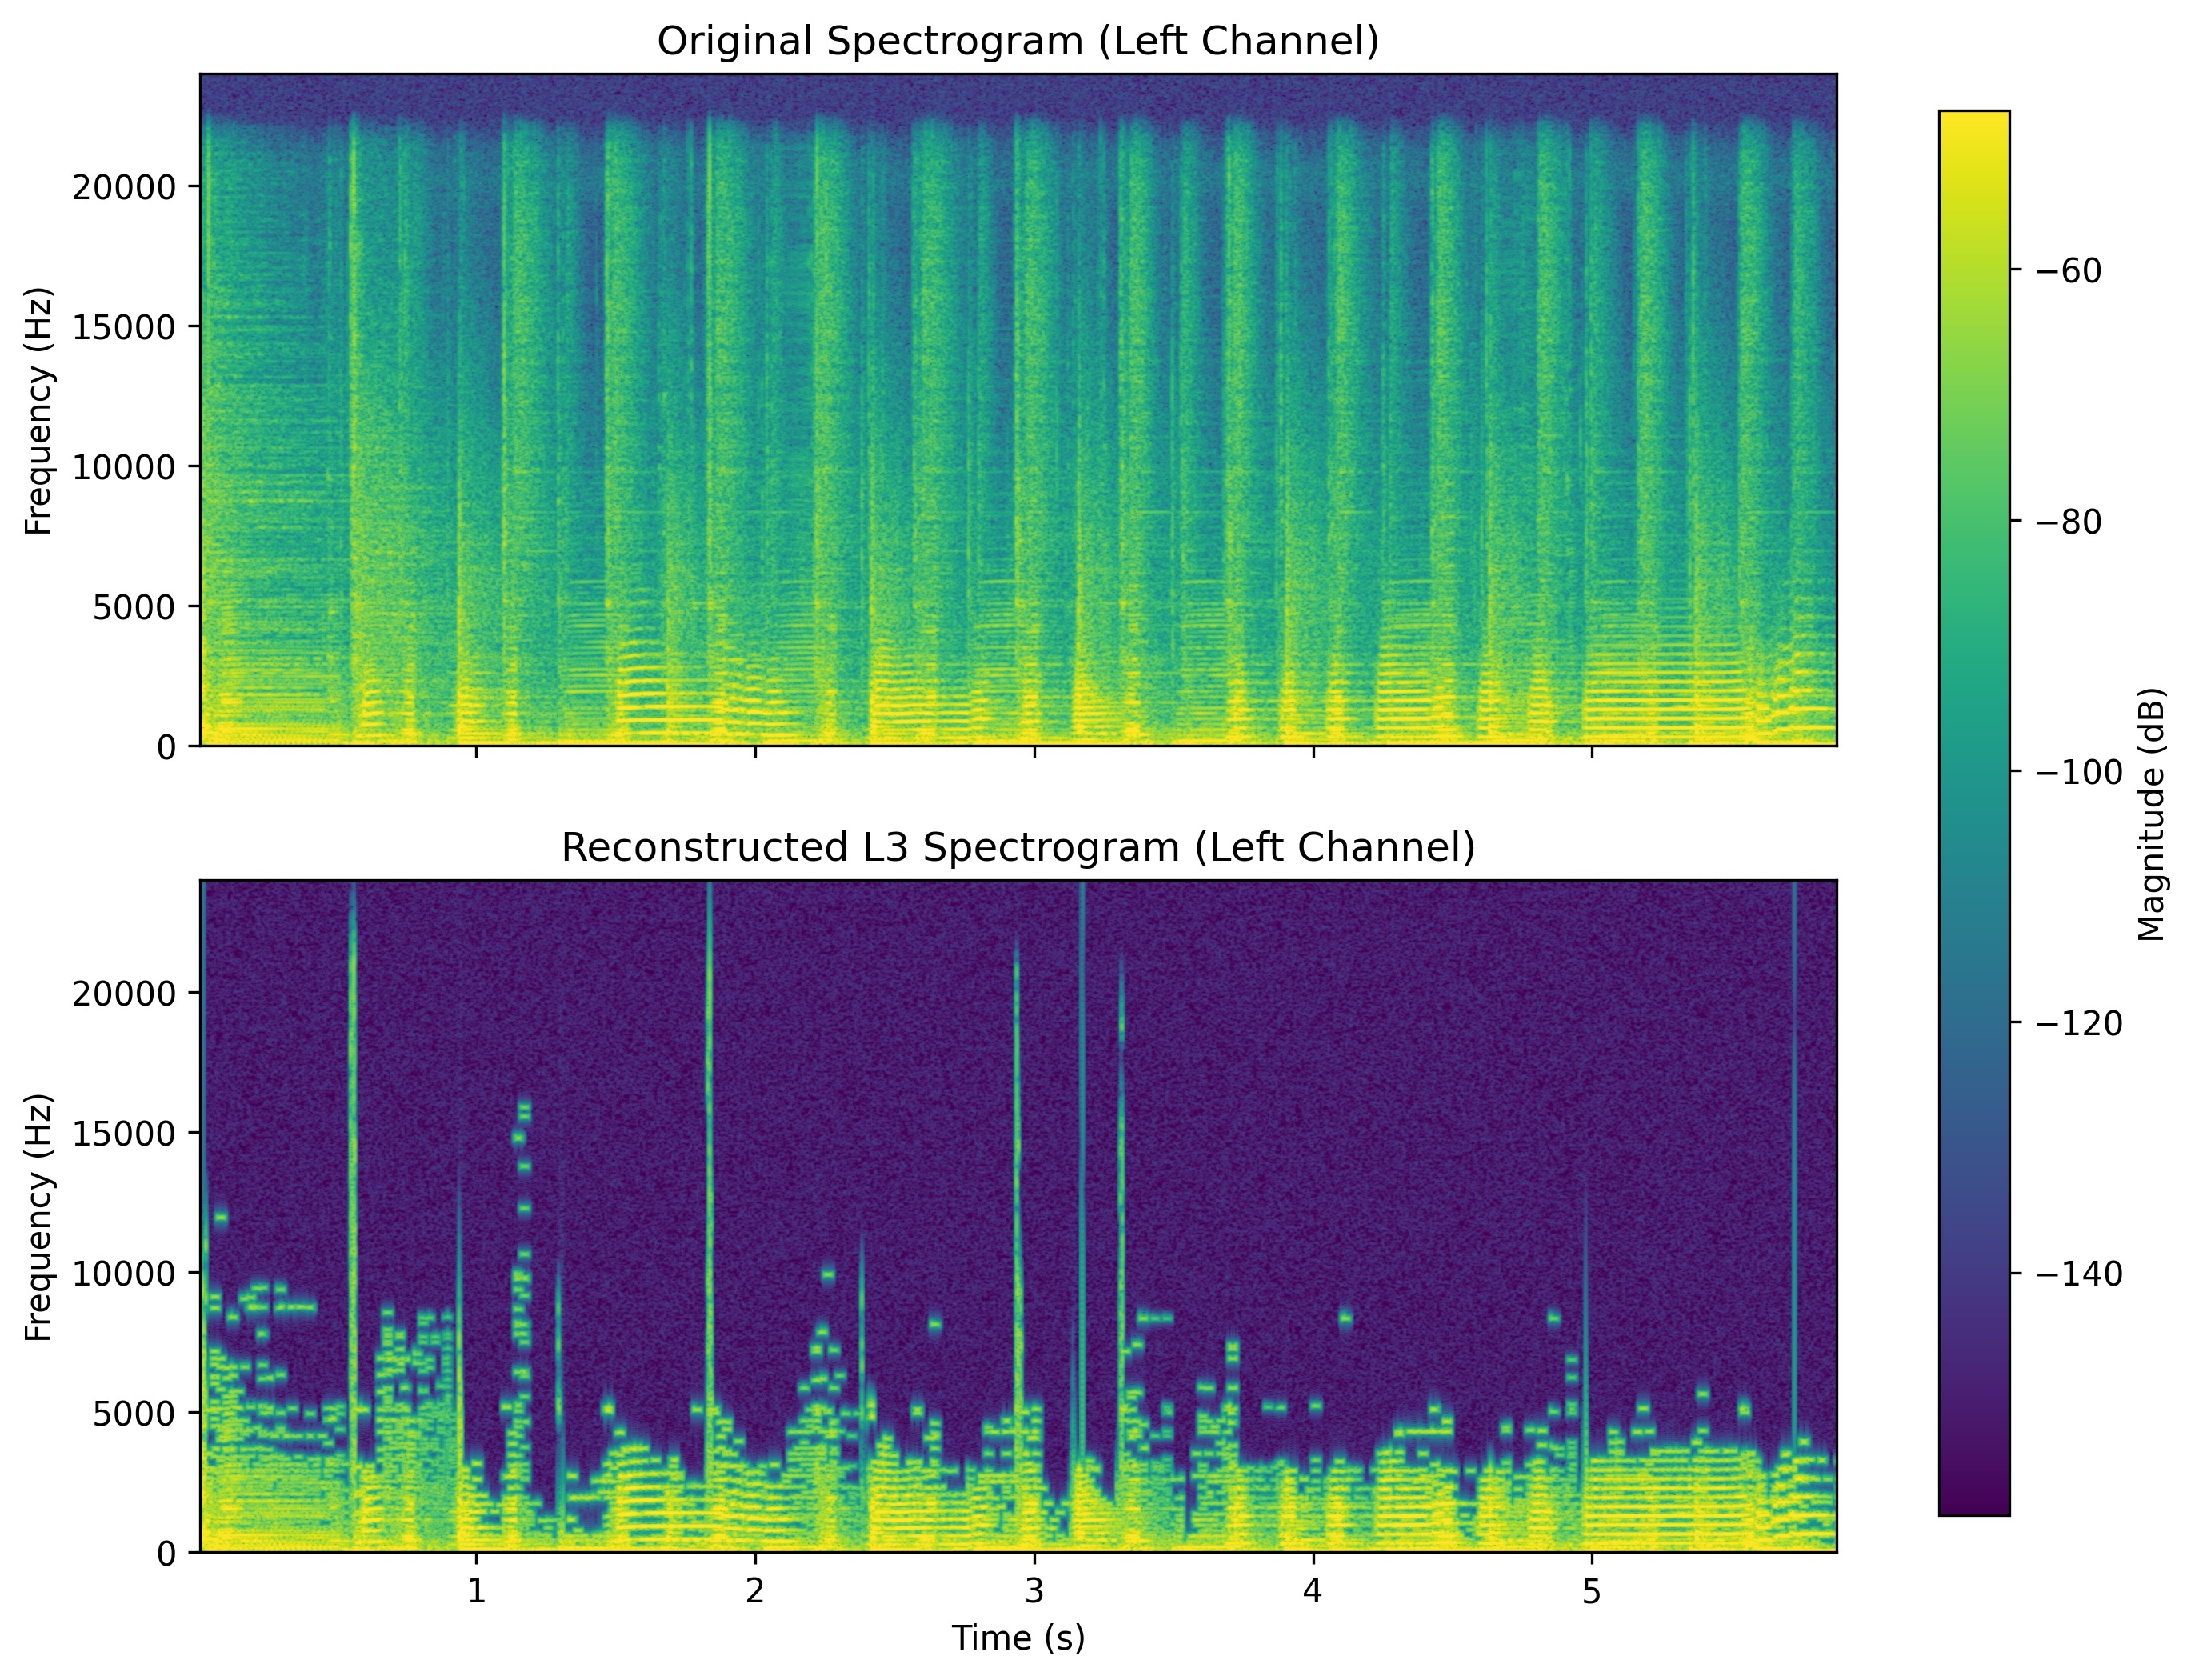
\includegraphics[width=0.8\textwidth]{spectrogram_comparison.png}
  \caption{Σύγκριση φασματογράμματος (COMPRESSION\_BIAS=57)}
  \label{fig:spectrogram_comparison}
\end{figure}

\clearpage

\section{Σύνοψη}

Συνοπτικά, η εργασία αυτή περιλαμβάνει την υλοποίηση και τη δοκιμή της κωδικοποίησης και αποκωδικοποίησης σύμφωνα με το απλοποιημένο πρότυπο AAC που περιγράφεται στην εκφώνηση. Συμπεριλαμβάνονται 3 διαφορετικά επίπεδα της υλοποίησης και ένας φάκελος με περισσότερα δοκιμαστικά αρχεία που αναδεικνύουν τη λειτουργία της τελικής εκδοχής του κωδικοποιητή-αποκωδικοποιητή. 

Κατά την εργασία αυτή, ο Βαπόρης Δημήτριος ανέλαβε την ανάπτυξη του κώδικα για τα πρώτα 2 επίπεδα, τον έλεγχο του κώδικα του 3ου επιπέδου και των δοκιμαστικών αρχείων και τη συγγραφή της συγκεκριμένης αναφοράς. Ο Ντελόπουλος Εμμανουήλ ανέλαβε τον έλεγχο του κώδικα των πρώτων 2 επιπέδων, την υλοποίηση του κώδικα του 3ου επιπέδου, τη συγγραφή των δοκιμαστικών αρχείων του φακέλου plotting και την παραγωγή των σχημάτων που παρουσιάστηκαν.

\clearpage
\listoffigures
\end{document}